\documentclass[10pt,twocolumn,letterpaper]{article}

\usepackage{cvpr}
\usepackage{times}
\usepackage{epsfig}
\usepackage{graphicx}
\usepackage{amsmath}
\usepackage{amssymb}
\usepackage[]{algorithm2e}

\usepackage{url}
\usepackage[italian]{babel}
\usepackage[utf8x]{inputenc}
\usepackage{listings}
\usepackage{color}
\usepackage[dvipsnames]{xcolor}
\usepackage[pagebackref=true,breaklinks=true,letterpaper=true,colorlinks,bookmarks=false]{hyperref}
\usepackage{blindtext}
\usepackage{enumitem}
\usepackage{calc}

\makeatletter
\newcommand{\DESCRIPTION@original@item}{}
\let\DESCRIPTION@original@item\item
\newcommand*{\DESCRIPTION@envir}{DESCRIPTION}
\newlength{\DESCRIPTION@totalleftmargin}
\newlength{\DESCRIPTION@linewidth}
\newcommand{\DESCRIPTION@makelabel}[1]{\llap{#1}}%
\newcommand{\DESCRIPTION@item}[1][]{%
  \setlength{\@totalleftmargin}%
       {\DESCRIPTION@totalleftmargin+\widthof{\textbf{#1 }}-\leftmargin}%
  \setlength{\linewidth}
       {\DESCRIPTION@linewidth-\widthof{\textbf{#1 }}+\leftmargin}%
  \par\parshape \@ne \@totalleftmargin \linewidth
  \DESCRIPTION@original@item[\textbf{#1}]%
}
\newenvironment{DESCRIPTION}
  {\list{}{\setlength{\labelwidth}{0cm}%
           \let\makelabel\DESCRIPTION@makelabel}%
   \setlength{\DESCRIPTION@totalleftmargin}{\@totalleftmargin}%
   \setlength{\DESCRIPTION@linewidth}{\linewidth}%
   \renewcommand{\item}{\ifx\@currenvir\DESCRIPTION@envir
                           \expandafter\DESCRIPTION@item
                        \else
                           \expandafter\DESCRIPTION@original@item
                        \fi}}
  {\endlist}
\makeatother

\cvprfinalcopy % *** Uncomment this line for the final submission

\def\cvprPaperID{****} % *** Enter the CVPR Paper ID here
\def\httilde{\mbox{\tt\raisebox{-.5ex}{\symbol{126}}}}

\newcommand{\Rplus}{\protect\hspace{-.1em}\protect\raisebox{.35ex}{\smaller{\smaller\textbf{+}}}}
\newcommand{\CC}{\mbox{C\Rplus\Rplus}\xspace}
\newcommand{\code}[1]{\texttt{#1}}
\renewcommand{\lstlistingname}{Codice}

\definecolor{mygray}{rgb}{0.5,0.5,0.5}
\definecolor{monokai@black}{HTML}{2C2C2A}
\definecolor{monokai@gray}{HTML}{524F52}
\definecolor{monokai@yellow}{HTML}{FDF5A9}
\definecolor{monokai@orange}{HTML}{FD971F}
\definecolor{monokai@red}{HTML}{DC322F}
\definecolor{monokai@magenta}{HTML}{D33682}
\definecolor{monokai@violet}{HTML}{F7208B}
\definecolor{monokai@blue}{HTML}{004C99}
\definecolor{monokai@green}{HTML}{009900}

\lstdefinestyle{monokaiJava}{
	frame=lines,
	language=Java,
	aboveskip=3mm,
	belowskip=3mm,
	showstringspaces=false,
	columns=flexible,
	basicstyle={\small\ttfamily},
	numbers=left,
	numberstyle=\tiny\color{monokai@black},
	numbersep=5pt,
	stepnumber=2,
	breaklines=true,
	breakatwhitespace=false,
	tabsize=2,
	numberstyle=\color{monokai@gray},
	keywordstyle=\color{monokai@violet},
	stringstyle=\color{monokai@green}\ttfamily,
	identifierstyle=\color{monokai@black},
	commentstyle=\color{monokai@blue},
	emphstyle=\color{monokai@red}
}

% Pages are numbered in submission mode, and unnumbered in camera-ready
\ifcvprfinal\pagestyle{empty}\fi
\begin{document}

%%%%%%%%% TITLE
\title{K-Means clustering con Apache Hadoop MapReduce}

\author{Filippo Mameli\\
filippo.mameli@stud.unifi.it\\
6222254
}

\maketitle

%%%%%%%%% ABSTRACT
\begin{abstract}
    La crescita dei volumi di dati da processare, ha reso necessario lo sviluppo
    di tecniche efficienti per la parallelizzazione dei metodi per
    l'analisi dei gruppi(clustering).
    In questo documento si presenta l'algoritmo di clustering K-Means utilizzando il
    modulo MapReduce del framework Apache Hadoop.
    Lo strumento migliora la scalabilità e le prestazioni dell'algoritmo su dati
    di grandi dimensioni distribuendo il carico computazionale e gli elementi da
    analizzare sull'hardware a disposizione.
\end{abstract}

% %%%%%%%%% BODY TEXT
\noindent\large\textbf{Permessi di distribuzione}\\
\indent L'autore di questa relazione permette che questo documento possa essere distribuito a tutti gli studenti UNIFI dei corsi futuri.
\section{Introduzione}
    Insieme allo sviluppo dell'information technology, è aumentata anche la
    quantità di dati da processare. In molti casi risulta impossibile assumere
    che una singola macchina possa mantenere nella memoria principale tutti
    i dati da analizzare. Per questo problema sono stati creati nuovi metodi
    per processare insiemi di dati contenenti numerosi oggetti.

    L'analisi dei gruppi (o clustering) ha delle tecniche che si fondano su
    assunzioni inattuabili su dataset di grandi dimensioni, per questo motivo
    uno dei più noti algoritmi di clustering K-Means è stato modificato basandosi
    sul modello di MapReduce, in modo tale da risolvere i problemi legati
    al volume di dati.

    In questo documento si presenta una possibile implementazione di K-Means
    basata su MapReduce utilizzando il framework Apache Hadoop. Nella Sezione
    \ref{baseKMeans} si introduce l'algoritmo generico di clustering per poi
    analizzare nella Sezione \ref{MRKMeans} la versione basata su MapReduce.
    Nella Sezione \ref{test} si mostrano invece i risultati derivanti dai
    test.

% -------------------------------------------------------------------------
\section{K-Means}
\label{baseKMeans}
    K-Means è un algoritmo di clustering molto noto. Questo prende in input un
    parametro $K$ e un numero $n$ di oggetti. L'obiettivo dell'algoritmo è quello di
    dividere gli $n$ oggetti in $K$ cluster in modo tale da massimizzare l'omogeneità
    degli elementi appartenenti ad un cluster. La similarità ad un
    cluster viene calcolata utilizzando il centroide. Questo è ricavato dalla media
    degli elementi appartenenti al cluster.

    Il primo passo dell'algoritmo è la creazione di $K$ centroidi in modo casuale.
    Questi rappresentano i centri dei cluster.

    Ciascuno degli $n$ oggetti
    viene assegnato al centroide più simile calcolando la distanza tra l'oggetto
    e il centro del cluster. Dopo l'assegnazione, i centri vengono ricalcolati
    utilizzando la media degli elementi del cluster.

    L'algoritmo continua a iterare sui nuovi centri e si ferma quando
    un determinato criterio di arresto viene soddisfatto.

\section{K-Means basato su MapReduce}
\label{MRKMeans}
    L'algoritmo K-Means utilizzando il modello di MapReduce è suddiviso in tre
    parti principali:
    \begin{itemize}
        \renewcommand{\labelitemi}{\scriptsize$\triangleright$}
        \item Map
        \item Combine
        \item Reduce
    \end{itemize}
    Nella parte di Map si assegna a ognuno degli $n$ oggetti uno dei $K$ centroidi.
    In modo da ridurre il carico di dati passati alla funzione di Reduce, la
    funzione di Combine calcola i risultati intermedi degli elementi
    che hanno lo stesso centroide. I dati poi passano alla funzione di Reduce che
    calcola la media degli elementi del centroide e assegna i nuovi valori.

    Alla fine della funzione di Reduce si controlla se il criterio di arresto viene
    soddisfatto. Se la condizione non è vera si continua a iterare ripartendo da Map
    operando sui centri riassegnati. L'algoritmo si interrompe nel caso in cui
    il requisito di arresto è soddisfatto.

\subsection{Implementazione con Apache Hadoop}
\label{hadoop}
    Il programma sviluppato processa l'algoritmo di K-Means su una serie di punti
    che appartengono ad uno spazio N-Dimensionale. I dati in input sono
    un insieme di file di testo che in ogni riga ha le coordinate di un punto.
    Ad esempio:
    $$1.17;2.5;3.895$$

    Il numero dei $K$ cluster viene specificato dall'utente ed è utilizzato
    per creare un file sequenziale. Il file contiene i centri generati in modo casuale
    e viene inizializzato prima dell'avvio del processo di MapReduce.

    Gli argomenti da indicare all'avvio del programma sono:
    \begin{itemize}
        \renewcommand{\labelitemi}{\scriptsize$\triangleright$}
        \item La cartella di input contenente i file di testo
        \item La cartella di output
        \item Il numero di $K$ centri
        \item Il numero di coordinate del punto
        \item Il valore che indica il limite per la convergenza dell'algoritmo
    \end{itemize}
    \subsubsection{Center e Point}
        Center e Point sono le classi su cui il processo di MapReduce lavora.
        Point è una classe che ha come unico campo la lista delle coordinate che
        descrivono il punto e implementa l'interfaccia \code{WritableComparable}.

        Center è una sottoclasse di Point, ma ha anche come campo un identificativo
        e il numero dei punti appartenenti al cluster associato al centro.\\
        I metodi di Center sono:
        \begin{DESCRIPTION}
            \item [divideCoordinates] Divide i valori delle coordinate per il numero di punti associati al centro
            \item [isConverged] Controlla se la distanza del centro rispetto ad un altro è minore del valore limite di convergenza
            \item [addNumOfPoints] Incrementa di un intero il numero di punti associati al centro
        \end{DESCRIPTION}
        \lstinputlisting[firstnumber= 16,firstline = 16, lastline = 20, style = monokaiJava, caption = Center, label = {code:center}]{../src/main/java/io/github/mameli/Center.java}
    \subsubsection{Map}
        La funzione di Map ha una parte di inizializzazione in cui ricava dal
        file sequenziale i centri che verranno poi inseriti in un ArrayList
        globale (Codice \ref{code:setupMap}).
        \lstinputlisting[firstnumber= 27,firstline = 27, lastline = 41, style = monokaiJava, caption = Setup di Map, label = {code:setupMap}]{../src/main/java/io/github/mameli/Map.java}

        Le istruzioni che esegue la funzione di Map sono mostrate nel
        Codice \ref{code:Map}. Nella prima parte del metodo si ricava le
        coordinate del punto dal file di input. Per ogni centro poi si calcola la
        distanza dal punto e infine si salva il centro più vicino all'elemento.
        \lstinputlisting[firstnumber= 44,firstline = 44, lastline = 64, style = monokaiJava, caption = Funzione Map, label = {code:Map}]{../src/main/java/io/github/mameli/Map.java}
    \subsubsection{Combine}
        La funzione Combine opera sulle coordinate dei punti che hanno associato lo
        stesso centro. Crea un oggetto Point che ha come valori le
        somme delle coordinate di tutti i punti e salva il numero di punti
        processati per aggiornare il valore \code{NumberOfPoints} del centro.

        Per esempio, con i punti (1,2,3) e (4,5,6) associati
        ad uno stesso centro si crea un oggetto Point che ha come coordinate
        (5,7,9) e si aggiorna il valore \code{NumberOfPoints} del centro a 2.

        \lstinputlisting[firstnumber= 16,firstline = 16, lastline = 32, style = monokaiJava, caption = Funzione Combine, label = {code:combine}]{../src/main/java/io/github/mameli/Combine.java}
    \subsubsection{Reduce}
        La funzione Reduce è molto simile a Combine. Infatti fa un ulteriore
        somma dei risultati parziali ricavati dalla funzione di Combine.
        Nel metodo \code{reduce} si popolano due HashMap: \code{newCenters} e \code{oldCenters}.
        Il primo contiene i centri che hanno come valori le somme delle coordinate
        dei punti a loro collegati e il numero di punti associati al cluster.
        Il secondo HashMap contiene i centri con i valori non aggiornati.
        \lstinputlisting[firstnumber= 29,firstline = 29, lastline = 58, style = monokaiJava, caption = Funzione Reduce, label = {code:reduce}]{../src/main/java/io/github/mameli/Reduce.java}

        Nella fase di cleanup si aggiorna concretamente i valori dei centri e
        si confrontano le nuove coordinate con quelle vecchie per vedere se
        la condizione di convergenza è soddisfatta.
        Per aggiornare i valori basta dividere le coordinate rispetto
        al numero dei punti del cluster. Questa operazione è eseguita
        richiamando la funzione \code{divideCoordinates}.

        La condizione di convergenza si divide in due vincoli:
        \begin{enumerate}
            \item Il centri che convergono (la distanza tra il vecchio
                valore e quello nuovo non supera il limite di threshold) sono maggiori o
                uguali al $90\%$.
            \item La media dei delle distanze tra i vecchi valori e quelli nuovi
                non supera il limite. La media è calcolata in questo modo:
                $$\sqrt{\frac{\sum{distanza^2}}{K}}$$
        Se uno di questi attributi viene soddisfatto allora un contatore globale identificato
        da \code{CONVERGE\_COUNTER.CONVERGED} viene incrementato.
        \end{enumerate}

        \lstinputlisting[firstnumber= 61,firstline = 61, lastline = 91, style = monokaiJava, caption = Cleanup, label = {code:cleanup}]{../src/main/java/io/github/mameli/Reduce.java}
    \subsubsection{Driver}
    \label{driver}
        La classe principale che contiene il main è \code{KMeans}. Questa contiene
        la configurazione e gestisce i job che eseguono il processo di MapReduce.
        La prima parte del metodo inizializza tutte le variabili necessarie
        per l'esecuzione dei job utilizzando gli argomenti dati in input.

        \lstinputlisting[firstnumber= 27,firstline = 27, lastline = 47, style = monokaiJava, caption = Setup di main, label = {code:setMain}]{../src/main/java/io/github/mameli/KMeans.java}

        Il processo di MapReduce vero e proprio si mostra nel Codice \ref{code:mapReduce}.
        Si inizializza tutte le classi utilizzate e gli elementi di
        input e di output. Dopo ogni \code{waitForCompletion} si controlla che
        il contatore contenente il valore che indica la condizione di convergenza.
        Se questa è diversa da 1 si deve continuare il processo e si cancella
        la cartella di output generata. Se è 1 invece si esce dal ciclo e si passa
        alla scrittura del risultato finale.

        \lstinputlisting[firstnumber= 49,firstline = 49, lastline = 70, style = monokaiJava, caption = Setup di main, label = {code:mapReduce}]{../src/main/java/io/github/mameli/KMeans.java}

        L'output finale è un file che viene generato con la classe Map su tutti
        i valori senza che i centri siano modificati (Codice \ref{code:mapOut}).\\

        \lstinputlisting[firstnumber= 71,firstline = 71, lastline = 83, style = monokaiJava, caption = Setup di main, label = {code:mapOut}]{../src/main/java/io/github/mameli/KMeans.java}

        \begin{figure}
            \centering
            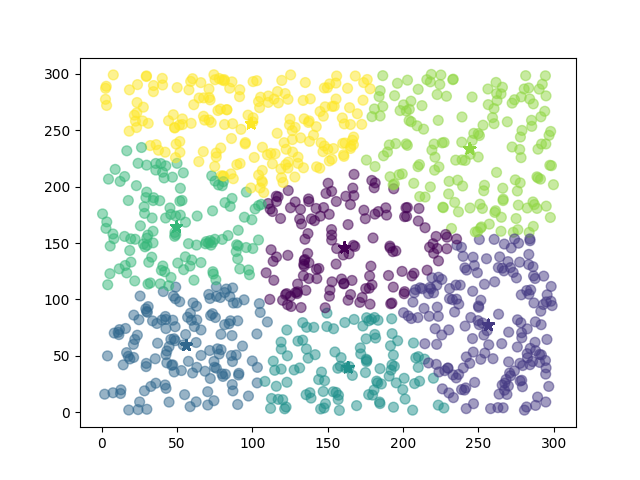
\includegraphics[width=\linewidth]{../img/2d.png}
            \caption{K = 7 e 1000 punti}
            \label{fig:fig1}
        \end{figure}
\section{Risultati sperimentali}
\label{test}
    Il programma è stato testato in locale e utilizzando i server con il servizio
    di Amazon Elastic Map Reduce (ERM).
    Oltre al programma Hadoop sono stati sviluppati degli script per la generazione
    di punti e per il plot dei risultati a due o tre dimensioni.

    Nella Figura \ref{fig:fig1} si mostra il risultato del processo su 1000 punti e
    7 cluster. Nella Figura \ref{fig:fig2} si aumenta il numero di punti a 10000 e i
    cluster a 25. In Figura \ref{fig:fig3} si mostra l'esempio di un risultato su 1000 punti
    a tre dimensioni con 5 cluster.

    \begin{figure}
        \centering
        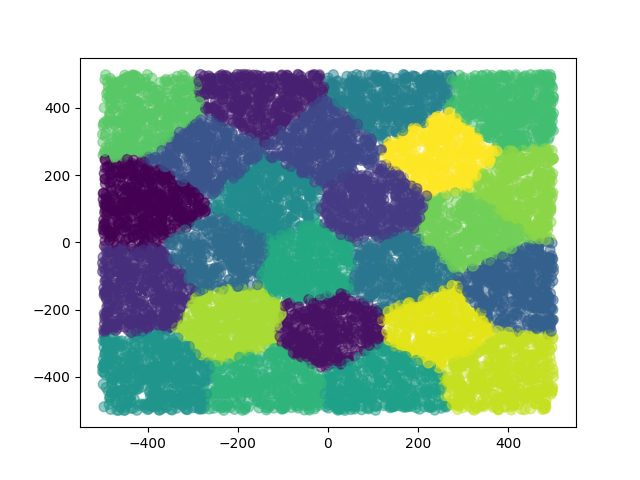
\includegraphics[width=\linewidth]{../img/2d2.png}
        \caption{K = 25 e 10000 punti}
        \label{fig:fig2}
    \end{figure}

    \begin{figure}
        \centering
        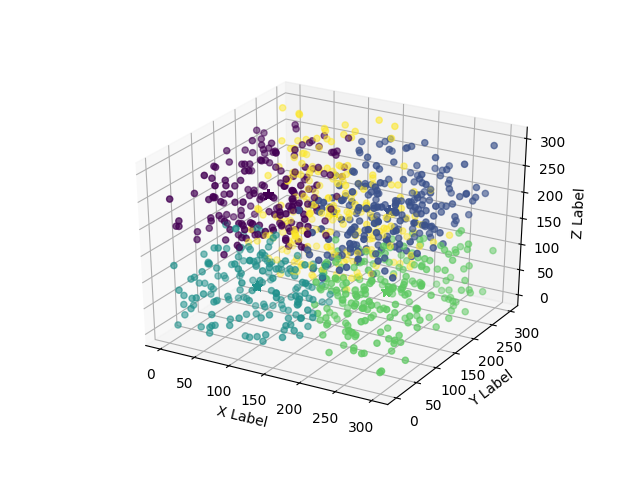
\includegraphics[width=\linewidth]{../img/3d.png}
        \caption{K = 5 e 1000 punti in 3d}
        \label{fig:fig3}
    \end{figure}

    \begin{figure}
        \centering
        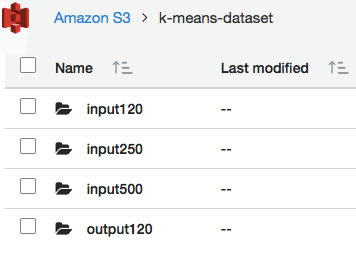
\includegraphics[width=\linewidth]{../img/s3.png}
        \caption{Dataset in S3}
        \label{fig:fig4}
    \end{figure}

    \begin{figure}
        \centering
        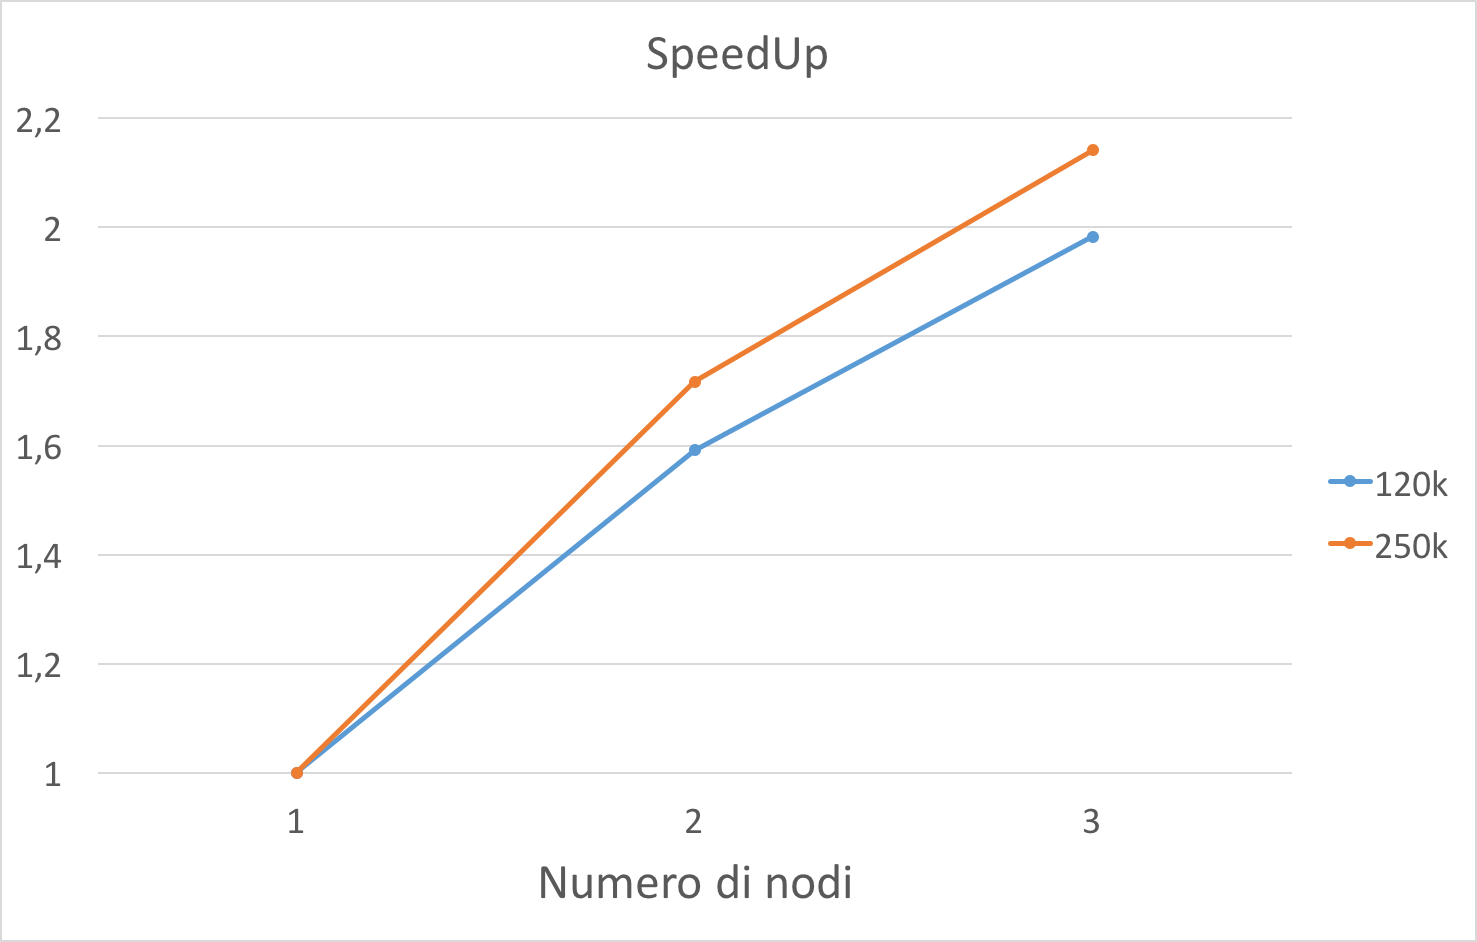
\includegraphics[width=\linewidth]{../img/speedUp.png}
        \caption{Speedup rispetto al numero di nodi}
        \label{fig:fig5}
    \end{figure}

    Usando il jar del progetto è stato possibile testare il processo anche su
    un ambiente completamente distribuito usufruendo del servizio di ERM.
    Caricando i dati su uno storage S3 (Figura \ref{fig:fig4}) sono state
    testate varie configuarazioni su dataset diversi.
    Sono stati processati in particolare cartelle contenenti i dati su un totale di
    120.000 punti e 250.000 punti su configurazioni con 1,2 e 3 nodi.
    Come si può vedere in Figura \ref{fig:fig5} lo speedup aumenta a seconda del
    numero di nodi, ma anche a seconda del carico di dati.

\section{Codice}
    Tutto il codice si può trovare nella repository di Github:
    \center{\url{https://github.com/mameli/k-means-hadoop}}





















\end{document}
